\documentclass[compress]{beamer}
\usepackage{ifthen,verbatim}

\newcommand{\isnote}{}
\xdefinecolor{lightyellow}{rgb}{1.,1.,0.25}
\xdefinecolor{darkblue}{rgb}{0.1,0.1,0.7}

%% Uncomment this to get annotations
%% \def\notes{\addtocounter{page}{-1}
%%            \renewcommand{\isnote}{*}
%% 	   \beamertemplateshadingbackground{lightyellow}{white}
%%            \begin{frame}
%%            \frametitle{Notes for the previous page (page \insertpagenumber)}
%%            \itemize}
%% \def\endnotes{\enditemize
%% 	      \end{frame}
%%               \beamertemplateshadingbackground{white}{white}
%%               \renewcommand{\isnote}{}}

%% Uncomment this to not get annotations
\def\notes{\comment}
\def\endnotes{\endcomment}

\setbeamertemplate{navigation symbols}{}
\setbeamertemplate{headline}{\mbox{ } \hfill
\begin{minipage}{5.5 cm}
\vspace{-0.75 cm} \small
\end{minipage} \hfill
\begin{minipage}{4.5 cm}
\vspace{-0.75 cm} \small
\begin{flushright}
Jim Pivarski \hspace{0.2 cm} \insertpagenumber\isnote/\pageref{numpages}
\end{flushright}
\end{minipage}\mbox{\hspace{0.2 cm}}\includegraphics[height=1 cm]{../cmslogo} \hspace{0.1 cm} \includegraphics[height=1 cm]{../tamulogo} \hspace{0.01 cm} \vspace{-1.05 cm}}

\begin{document}

\scriptsize

\begin{frame}
\frametitle{Sawtooth effect (1/2)}

\begin{columns}
\column{0.5\linewidth}

\vspace{0.2 cm}
\begin{itemize}\setlength{\itemsep}{0.1 cm}
\item Alignment plots revealed $r\phi$ residual vs.~$\phi$ structure inside chambers
\item Entrance angle is correlated with $\phi$ (i.e.~$x$) and more relevant \mbox{for chambers;\hspace{-1 cm}}
\textcolor{red}{correlation in data} is \mbox{stronger (below)\hspace{-1 cm}}
\item \textcolor{blue}{Collisions MC} doesn't \mbox{show the effect\hspace{-0.5 cm}} (shows a radial
  displacement instead: confirmed in orthogonal residuals, a separate
  \mbox{problem involving the propagator?)\hspace{-3 cm}}
\end{itemize}

\column{0.5\linewidth}
\includegraphics[height=\linewidth, angle=90]{alignmentplots_example2.pdf}
\end{columns}

\begin{center}
Focus on just one chamber (wheel 0, station 1, sector 10), $p_T > 40$~GeV

\mbox{ } \hfill \includegraphics[width=0.37\linewidth]{original_sawtooth.pdf} \hfill \includegraphics[width=0.37\linewidth]{vstrackangle_sawtooth.pdf} \hfill \begin{minipage}{1.6 cm} \vspace{-3 cm} \tiny data include latest $\vec{B}(\vec{x})$ map and superlayer radial corrections \end{minipage}\mbox{ }
\end{center}

\end{frame}

\begin{frame}
\frametitle{Sawtooth effect (2/2)}

\begin{columns}
\column{0.7\linewidth}
\begin{itemize}\setlength{\itemsep}{0.25 cm}
\item Seems to derive from an understandable effect: \mbox{$x$ residuals\hspace{-1 cm}}
  {\it should} be correlated with track-segment \mbox{angle difference\hspace{-1 cm}}
\item But an unexplained correlation between the \mbox{angle difference\hspace{-0.75 cm}} and
  the angle links $x$ residuals to angle \mbox{(sawtooth effect)\hspace{-1 cm}}
\item Second correlation is not understood and not in MC,

independent of $q$ and $p_T$ (unrelated to $\vec{B}$ and $dE/dx$)

\item Also, same effect in $y$ residuals vs.\ $dx/dz$ angle!

\item Ugo, Pablo, and Alecia are \mbox{investigating with segments and tracks\hspace{-5 cm}}

\end{itemize}

\column{0.3\linewidth}
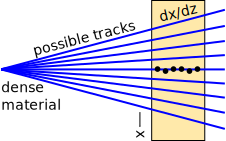
\includegraphics[width=\linewidth]{understandable_correlation_diagram.pdf}
\end{columns}

\vfill
\begin{columns}
\column{0.33\linewidth}
\mbox{ } \hfill \textcolor{darkblue}{this makes sense} \hfill \mbox{ }

\includegraphics[width=\linewidth]{understandable_effect.pdf}

\column{0.33\linewidth}
\textcolor{darkblue}{why is this correlated \mbox{in data?\hspace{-1 cm}}}

\includegraphics[width=\linewidth]{strange_correlation.pdf}

\column{0.33\linewidth}
\hfill \textcolor{darkblue}{and why do we see same} \hspace{0.07 cm}

\hfill \textcolor{darkblue}{effect on other parameter?}

\includegraphics[width=\linewidth]{evenstranger_sawtooth.pdf}
\end{columns}
\label{numpages}
\end{frame}

\end{document}
